\documentclass{article}
\usepackage{graphicx}
\usepackage{fancyhdr}
\pagestyle{fancy}
\lhead{Ruicheng Wu}
\rhead{07/15/2017}
\chead{Homework 7}

\begin{document}
1.

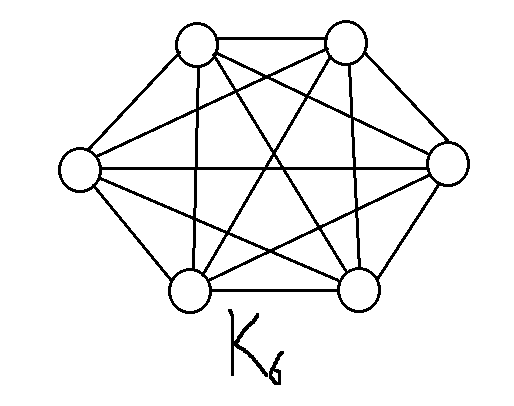
\includegraphics[scale=.3]{HW7_k6.png}

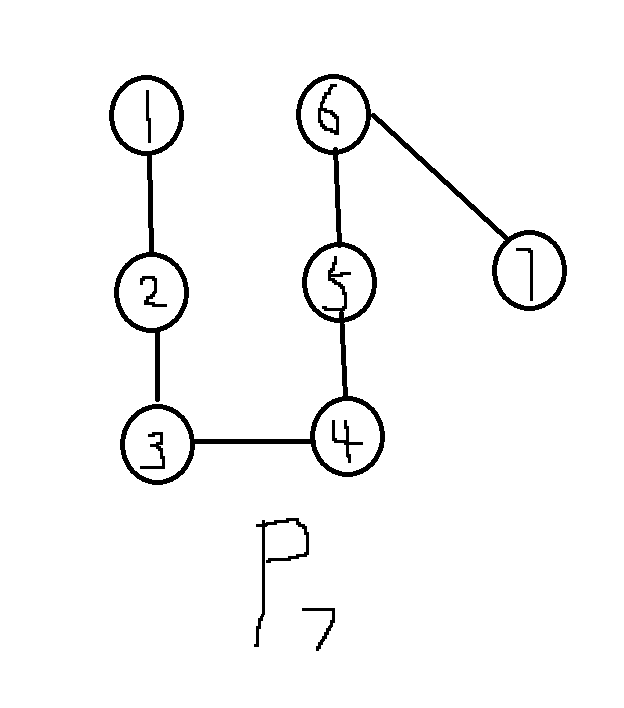
\includegraphics[scale=.3]{HW7_p7.png}

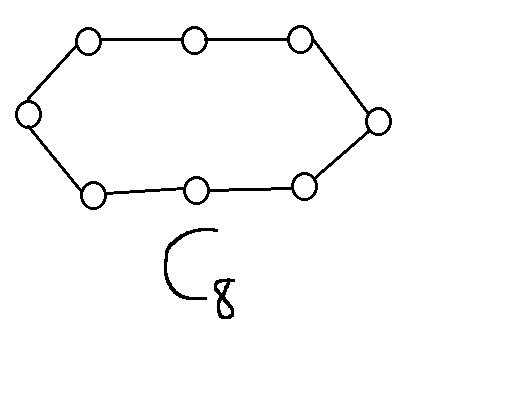
\includegraphics[scale=.3]{HW7_c8.png}

2.

A and B is isomorphic,

First we examine the degree sequence of each:

A:{$4,4,4,4,3,3$}
B:{$4,4,4,4,3,3$}

Next,simply relabel vertices in B : 3 to 2,4 to 5(of course 2 to 3,5 to 4):

The number inside of parentheses is the original label:
 
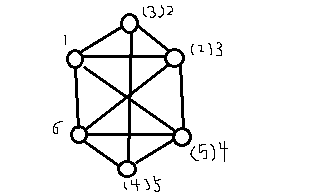
\includegraphics[scale=.7]{HW7_2a.png}

We can see it is obviously the same graph as A.So they are isomorphic.

C and D are not isomorphic,although they have same degree sequence.It is very obviously that the edge between 1 and 5, 7 and 3 in C can never be relabeled as 2 to 7 , 3 to 8 in D. This is just because 5 and 7 are not adjacent to each other in C;while in D,7 and 8 are adjacent to each other,there is no way that C and D can be isomorphic graph.

3.

Given n labeled vertices,think it as a board with n points.Every time we just choose 2 points from those n points to construct the edge.There will be overcounting on some isomorphic graph. Since the question treat them as different graph,so  the total number of graph is just : $2^{C(n,2)}$

4.

(a)No such graph exist,the total number of degree is odd.According to the definition,the total degree of a graph is even.So no such graph exist.

(b)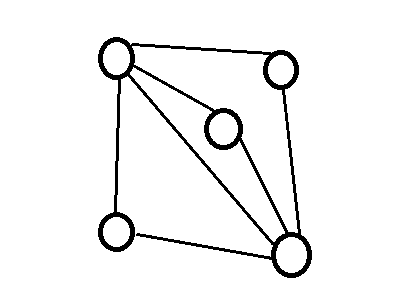
\includegraphics[scale=.3]{HW7_4b.png}

(c)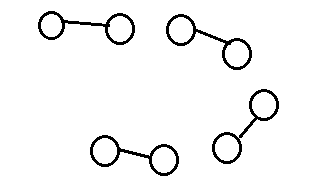
\includegraphics[scale=.3]{HW7_4c.png}

(d)No such graph exist,same as (a),the total degree is odd and also its first vertex has degree of 7,which is impossible to construct 7 edges from that one to rest vertices while the sum of rest is just 6.

5.

There are 6 vertices in total, so we need a 6 x 6 matrix:

\[
\left[ \begin {array}{ccc}
010000\\
101000\\
010110\\
001001\\
001001\\
000110
\end{array} \right]
\]

\end{document}

